%% LyX 2.0.2 created this file.  For more info, see http://www.lyx.org/.
%% Do not edit unless you really know what you are doing.
\documentclass[spanish]{article}
\usepackage[T1]{fontenc}
\usepackage[latin9]{inputenc}
\usepackage{float}
\usepackage{textcomp}
\usepackage{amstext}
\usepackage{amssymb}
\usepackage{graphicx}
\usepackage{esint}

\makeatletter

%%%%%%%%%%%%%%%%%%%%%%%%%%%%%% LyX specific LaTeX commands.
%% Because html converters don't know tabularnewline
\providecommand{\tabularnewline}{\\}

%%%%%%%%%%%%%%%%%%%%%%%%%%%%%% User specified LaTeX commands.
\date{}

\makeatother

\usepackage{babel}
\addto\shorthandsspanish{\spanishdeactivate{~<>}}

\begin{document}

\title{Informe de Lectura\\
por\\
Alejandro Mesa G�mez\\
\texttt{almego95@gmail.com}~\\
\texttt{}~\\
ENERGIA RELATIVISTA}

\maketitle
Para obtener la forma relativista del teorema del trabajo y la energ�a,
empezamos con la definici�n del trabajo realizado sobre una particula
por una fuerza F y empleamos la definici�n de fuerza relativista:

\begin{equation}
W=\int_{x}^{x2}F\, dx=\int_{x1}^{x2}\frac{dp}{dt}\: dx\label{eq:trabajo}
\end{equation}


\begin{table}[H]
\centering{}%
\begin{tabular}{r@{\extracolsep{0pt}.}l|r@{\extracolsep{0pt}.}l|r@{\extracolsep{0pt}.}l}
\multicolumn{2}{c}{} & \multicolumn{2}{c}{} & \multicolumn{2}{c}{}\tabularnewline
\hline 
\hline 
\multicolumn{2}{c|}{Cantidad} & \multicolumn{2}{c|}{Cl�sica} & \multicolumn{2}{c}{Relativista}\tabularnewline
\hline 
\hline 
\multicolumn{2}{c|}{Masa (Inercia)} & \multicolumn{2}{c|}{Invariante} & \multicolumn{2}{c}{Relativa}\tabularnewline
\multicolumn{2}{c|}{Energ�a mec�nica} & \multicolumn{2}{c|}{$E=K+U$} & \multicolumn{2}{c}{$E=\gamma mc^{2}$}\tabularnewline
\multicolumn{2}{c|}{Energia Cin�tica} & \multicolumn{2}{c|}{$K=mv^{2}/2$} & \multicolumn{2}{c}{$K=mc^{2}(\gamma-1)$}\tabularnewline
\hline 
\end{tabular}\caption{\label{tab:cuadro1}Comparacion de distintas cantidades mec�nicas
en la teoria Newtoniana (cl�sica) y en la relatividad. Aqu� $\gamma=(1-v^{2}/c^{2})^{-1/2}$}
\end{table}


para la fuerza y el movimiento a lo largo del eje x. Primero evaluamos
$dp/dt$:

\[
\frac{dp}{dt}=\frac{d}{dt}\frac{mu}{\sqrt{1-\frac{u^{2}}{c^{2}}}}=\frac{m(du/dt)}{(1-\frac{u^{2}}{c^{2}})^{3/2}}\: con\: u<c
\]


si sustituimos esta expresion para $dp/dt$ y $dx=udt$ en la ecuaci�n
(\ref{eq:trabajo}), se obtiene

\[
W=\int_{x1}^{x2}\frac{m(du/dt)udt}{(1-\frac{u^{2}}{c^{2}})^{3/2}}=\int_{0}^{u}\frac{u}{(1-\frac{u^{2}}{c^{2}})^{3/2}}du
\]


al evaluar la integral encontramos que\\
\\
\\
\begin{figure}[H]
\begin{centering}
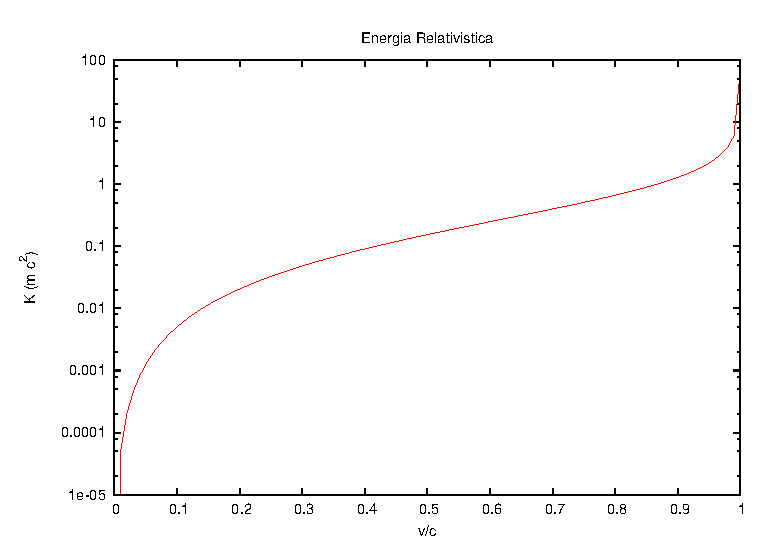
\includegraphics{K}
\par\end{centering}

\caption{\label{fig:figura1}Energia cin�tica relativistica como funcion de
la velocidad}


\end{figure}


\begin{equation}
W=\frac{mc\text{\texttwosuperior}}{\sqrt{1-\frac{u\text{\texttwosuperior}}{c\text{\texttwosuperior}}}}-mc\text{\texttwosuperior}\label{eq:ecuacion2}
\end{equation}


como el trabajo realizadopor una fuerza que act�a sobre una part�cula
es igual al cambio de la energia cin�tica, entonces el trabajo es
igual a la energia cinetica relativistica$K$:\\


\begin{equation}
K=\frac{mc^{2}}{\sqrt{1-\frac{u^{2}}{c^{2}}}}-mc^{2}=\gamma mc^{2}-mc^{2}\label{eq:ecuacion 3}
\end{equation}
\\


En la tabla(\ref{tab:cuadro1}) se comparan distintas cantidades f�sicas
segun la f�sica clasica y la relativista.

A bajas velocidades donde $u/c\ll1$ la ecuacion debe reducirse a
la expresi�n clasica $K=\frac{1}{2}mv\text{\texttwosuperior}$. Podemos
verificar esto con la expansi�n del binomio\\
\\
\\
 $(1-x)^{-1/2}\thickapprox1+\frac{1}{2}x^{2}+....$La sustituci�n
de esto en la ecuaci�n produce

\[
K=mc^{2}(1+\frac{1}{2}\frac{u^{2}}{c^{2}}+...)-mc^{2}=\frac{1}{2}mu^{2}
\]


lo cual concuerda con el resultado cl�sico.%
\footnote{Tomado de \textbf{\textit{F�sica, Tomo II. }}\textit{Raymon A. Serway,
}Sec. 39.7%
}

la figura(\ref{fig:figura1}) muestra la energia cin�tica como funcion
de la velocidad.
\end{document}
